\documentclass[a4paper,11pt]{article}
\usepackage[utf8]{inputenc}
\usepackage{minted}
\usepackage{amsmath}
\usepackage{float}
\usepackage[symbol]{footmisc}
\usepackage{graphicx}
\usepackage[toc,page]{appendix}

\graphicspath{{./figures/}}
\renewcommand{\thefootnote}{\fnsymbol{footnote}}

\title{\textbf{6. Trees}}
\author{Kristiāns Vinters}
\date{Fall 2023}

\begin{document}
    \maketitle
    \section*{Introduction}

    I solved the assignment in Go. I used Go because I want to become more familiar with it. Source code and benchmark data is available on GitHub\footnote[1]{https://github.com/Phanty133/id1021/tree/master/6-trees}.

    \section*{Implementation}

    I implemented the binary tree with generic structs. The key has a type constraint of \mintinline{go}{cmp.Ordered}, which is an interface that requires the type to implement the \mintinline{go}{cmp.Ordered} method, which means that the type must be comparable. The value can be any type.

    \begin{minted}{go}
type BinaryTreeNode[K cmp.Ordered, V any] struct {
    Key   K
    Val   V
    Left  *BinaryTreeNode[K, V]
    Right *BinaryTreeNode[K, V]
}

type BinaryTree[K cmp.Ordered, V any] struct {
    Root *BinaryTreeNode[K, V]
}
    \end{minted}

    The add and lookup methods were implemented as private methods on the \mintinline{go}{BinaryTreeNode} struct, while \mintinline{go}{BinaryTree} has public methods that call the private methods on the root node.

    \begin{minted}{go}
func (t *BinaryTree[K, V]) Lookup(key K) (V, bool) {
    return t.Root.lookup(key)
}

func (node *BinaryTreeNode[K, V]) lookup(key K) (V, bool) {
    if node == nil {
        var zero V
        return zero, false
    }

    if node.Key == key {
        return node.Val, true
    }

    if key < node.Key {
        return node.Left.lookup(key)
    }

    return node.Right.lookup(key)
}

func (t *BinaryTree[K, V]) Add(key K, val V) {
    if t.Root == nil {
        t.Root = NewBinaryTreeNode(key, val)
        return
    }

    t.Root.add(key, val)
}

// Returns true if the key was added, false if it was updated.
func (node *BinaryTreeNode[K, V]) add(key K, val V) bool {
    if node.Key == key {
        node.Val = val
        return false
    }

    if key < node.Key {
        if node.Left == nil {
            node.Left = NewBinaryTreeNode(key, val)
            return true
        }

        return node.Left.add(key, val)
    }

    if node.Right == nil {
        node.Right = NewBinaryTreeNode(key, val)
        return true
    }

    return node.Right.add(key, val)
}
    \end{minted}

    For depth-first traversal, I was not able to use an iterator, as Go does not have them. Instead, I used a goroutine and a function that returns a channel that can be made to act in a similar way to an iterator.

    \begin{minted}{go}
func (t *BinaryTree[K, V]) DepthFirstIterator() <-chan *BinaryTreeNode[K, V] {
    ch := make(chan *BinaryTreeNode[K, V])

    go func() {
        t.Root.depthFirstIterator(ch)
        close(ch)
    }()

    return ch
}

func (node *BinaryTreeNode[K, V]) depthFirstIterator(ch chan<- *BinaryTreeNode[K, V]) {
    if node == nil {
        return
    }

    node.Left.depthFirstIterator(ch)
    ch <- node
    node.Right.depthFirstIterator(ch)
}
    \end{minted}

    The idea is that each node sends itself to the channel, which blocks further execution in the goroutine until the channel is read from. Compared to a normal iterator, this adds concurrency to the program, which means that the return value and the traversal to the next node can be processed concurrently. The returned channel can be iterated over with a simple \mintinline{go}{for range} loop. If a node is added during iteration, depending on the key, it may or may not be iterated over. If the key is less than the current node's key, it will not be iterated over, as it will be added to a subtree that has already been iterated over. If the key is greater than the current node's key, it will be iterated over, as it will be added to a subtree that has not yet been iterated over.

    \begin{minted}{go}
tree := tree.NewBinaryTree[int, int]()

tree.Add(5, 5)
tree.Add(3, 3)
tree.Add(7, 7)
tree.Add(2, 2)

for node := range tree.DepthFirstIterator() {
    fmt.Printf("%d ", node.Val)
}

// Output: 2 3 5 7
    \end{minted}

    \section*{Benchmarks}

    I benchmarked the add and lookup methods. I initialized N random key, value pairs that were then added to a tree for $N \in \{100, 1000, 5000, 10000$, $50000, 100000, 500000, 1000000\}$. Then I added 1000 more random nodes 250 times for each size (Generating a new tree for every repeat). Outputs were written to a CSV file, which was then further analyzed in LibreOffice Calc. I measured min, max, median, and mean execution times.

    \begin{figure}[H]
        \centering
        \begin{tabular}{c|c|c|c|c}
            N & Mean, $\mu s$ & Median, $\mu s$ & Min, $\mu s$ & Max, $\mu s$ \\
            \hline
            \hline
            100 & 0.08 & 0.07 & 0.07 & 0.42 \\
            \hline
            1000 & 0.09 & 0.08 & 0.08 & 0.25 \\
            \hline
            10000 & 0.13 & 0.12 & 0.11 & 0.37 \\
            \hline
            100000 & 0.23 & 0.22 & 0.20 & 0.41 \\
            \hline
            1000000 & 0.61 & 0.59 & 0.54 & 0.92 \\
        \end{tabular}

        \caption{Sample data for 1000 adds}
    \end{figure}

    \begin{figure}[H]
        \centering
        \begin{tabular}{c|c|c|c|c}
            N & Mean, $\mu s$ & Median, $\mu s$ & Min, $\mu s$ & Max, $\mu s$ \\
            \hline
            \hline
            100 & 0.04 & 0.04 & 0.03 & 0.05 \\
            \hline
            1000 & 0.06 & 0.06 & 0.06 & 0.20 \\
            \hline
            10000 & 0.10 & 0.09 & 0.09 & 0.23 \\
            \hline
            100000 & 0.22 & 0.21 & 0.19 & 0.59 \\
            \hline
            1000000 & 0.67 & 0.65 & 0.52 & 1.22 \\
        \end{tabular}

        \caption{Sample data for 1000 lookups}
    \end{figure}

    \begin{figure}[H]
        \centering
        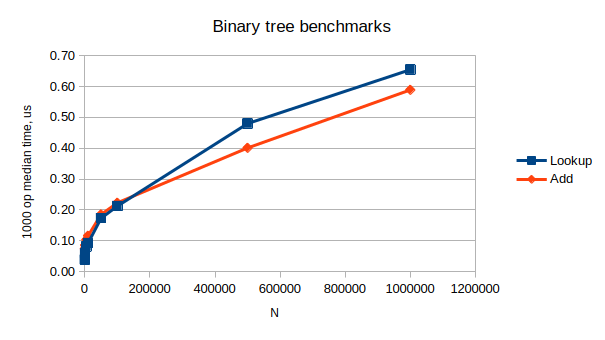
\includegraphics[width=\textwidth]{bt}
        \caption{Lookup and Add method median execution times}
    \end{figure}

    Lookup and add appear to have similar complexities, however, when graphing against $log_2 N$, which is the expected average case complexity, the trend is not linear. This is likely due to the fact that the randomly generated trees are not balanced. The worst case complexity is $O(N)$ because a tree can degenerate to a simple linked list. It can be seen that the actual execution times are between the average and worst case complexities. Had the tree been created with an ordered set of keys, the tree would have been balanced, and the actual execution times would have been closer to the average case complexity.

    \begin{figure}[H]
        \centering
        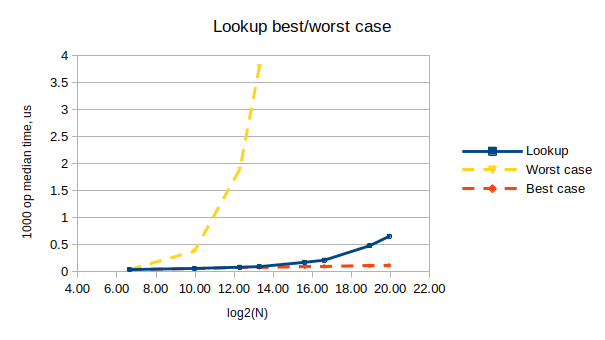
\includegraphics[width=\textwidth]{lookup}
        \caption{Actual lookup median execution time vs best and worst case complexities, using $N=100$ to calculate the constant factor.}
    \end{figure}
\end{document}